\chapter{Descritores de imagens}

Tendo em vista que as imagens, devido a grade quantidade de informações
contidas em sua representação, não servem como entrada para uma rede de Kohonen,
é necessário extrair delas um conjunto resumido e mensurável de características
que possam servir de entrada para rede. É sobre a extração deste conjunto de
características que trata este capítulo. Serão abordados os descritores
escolhidos para caracterizar uma imagem e também todo o tratamento que a imagem
sofre até que estes descritores possam ser extraídos.

\section{Conceitos introdutórios sobre imagens digitais}\label{sec:conc_intro}

Antes de inicar qualquer discução a respeito da caracterização e agrupamento de
imagens é necessário discorrer sob o modo com as imagens são representadas
computacionalmente, os termos comumente empregados nestas representações e,
em particular, estabelecer quais destas representações serão adotadas neste
trabalho.

Existe basicamente duas formas de representação computacional de imagens,
mapa de bits (\textit{bitmap}): uma matriz de pontos (\textit{pixels}) que representam cores;
ou vetoriais: um conjunto de descrições de formas geométricas, cores e texturas
que, precisamente por serem equações vetoriais ou trasformações matemáticas,
não perdem a qualidade quando redimensionadas ou rotacionadas; a
comparação entre estas duas representações pode ser observada na
Figura \ref{fig:vetor_x_bitmap}.

\begin{figure}[H]
  \begin{center}
    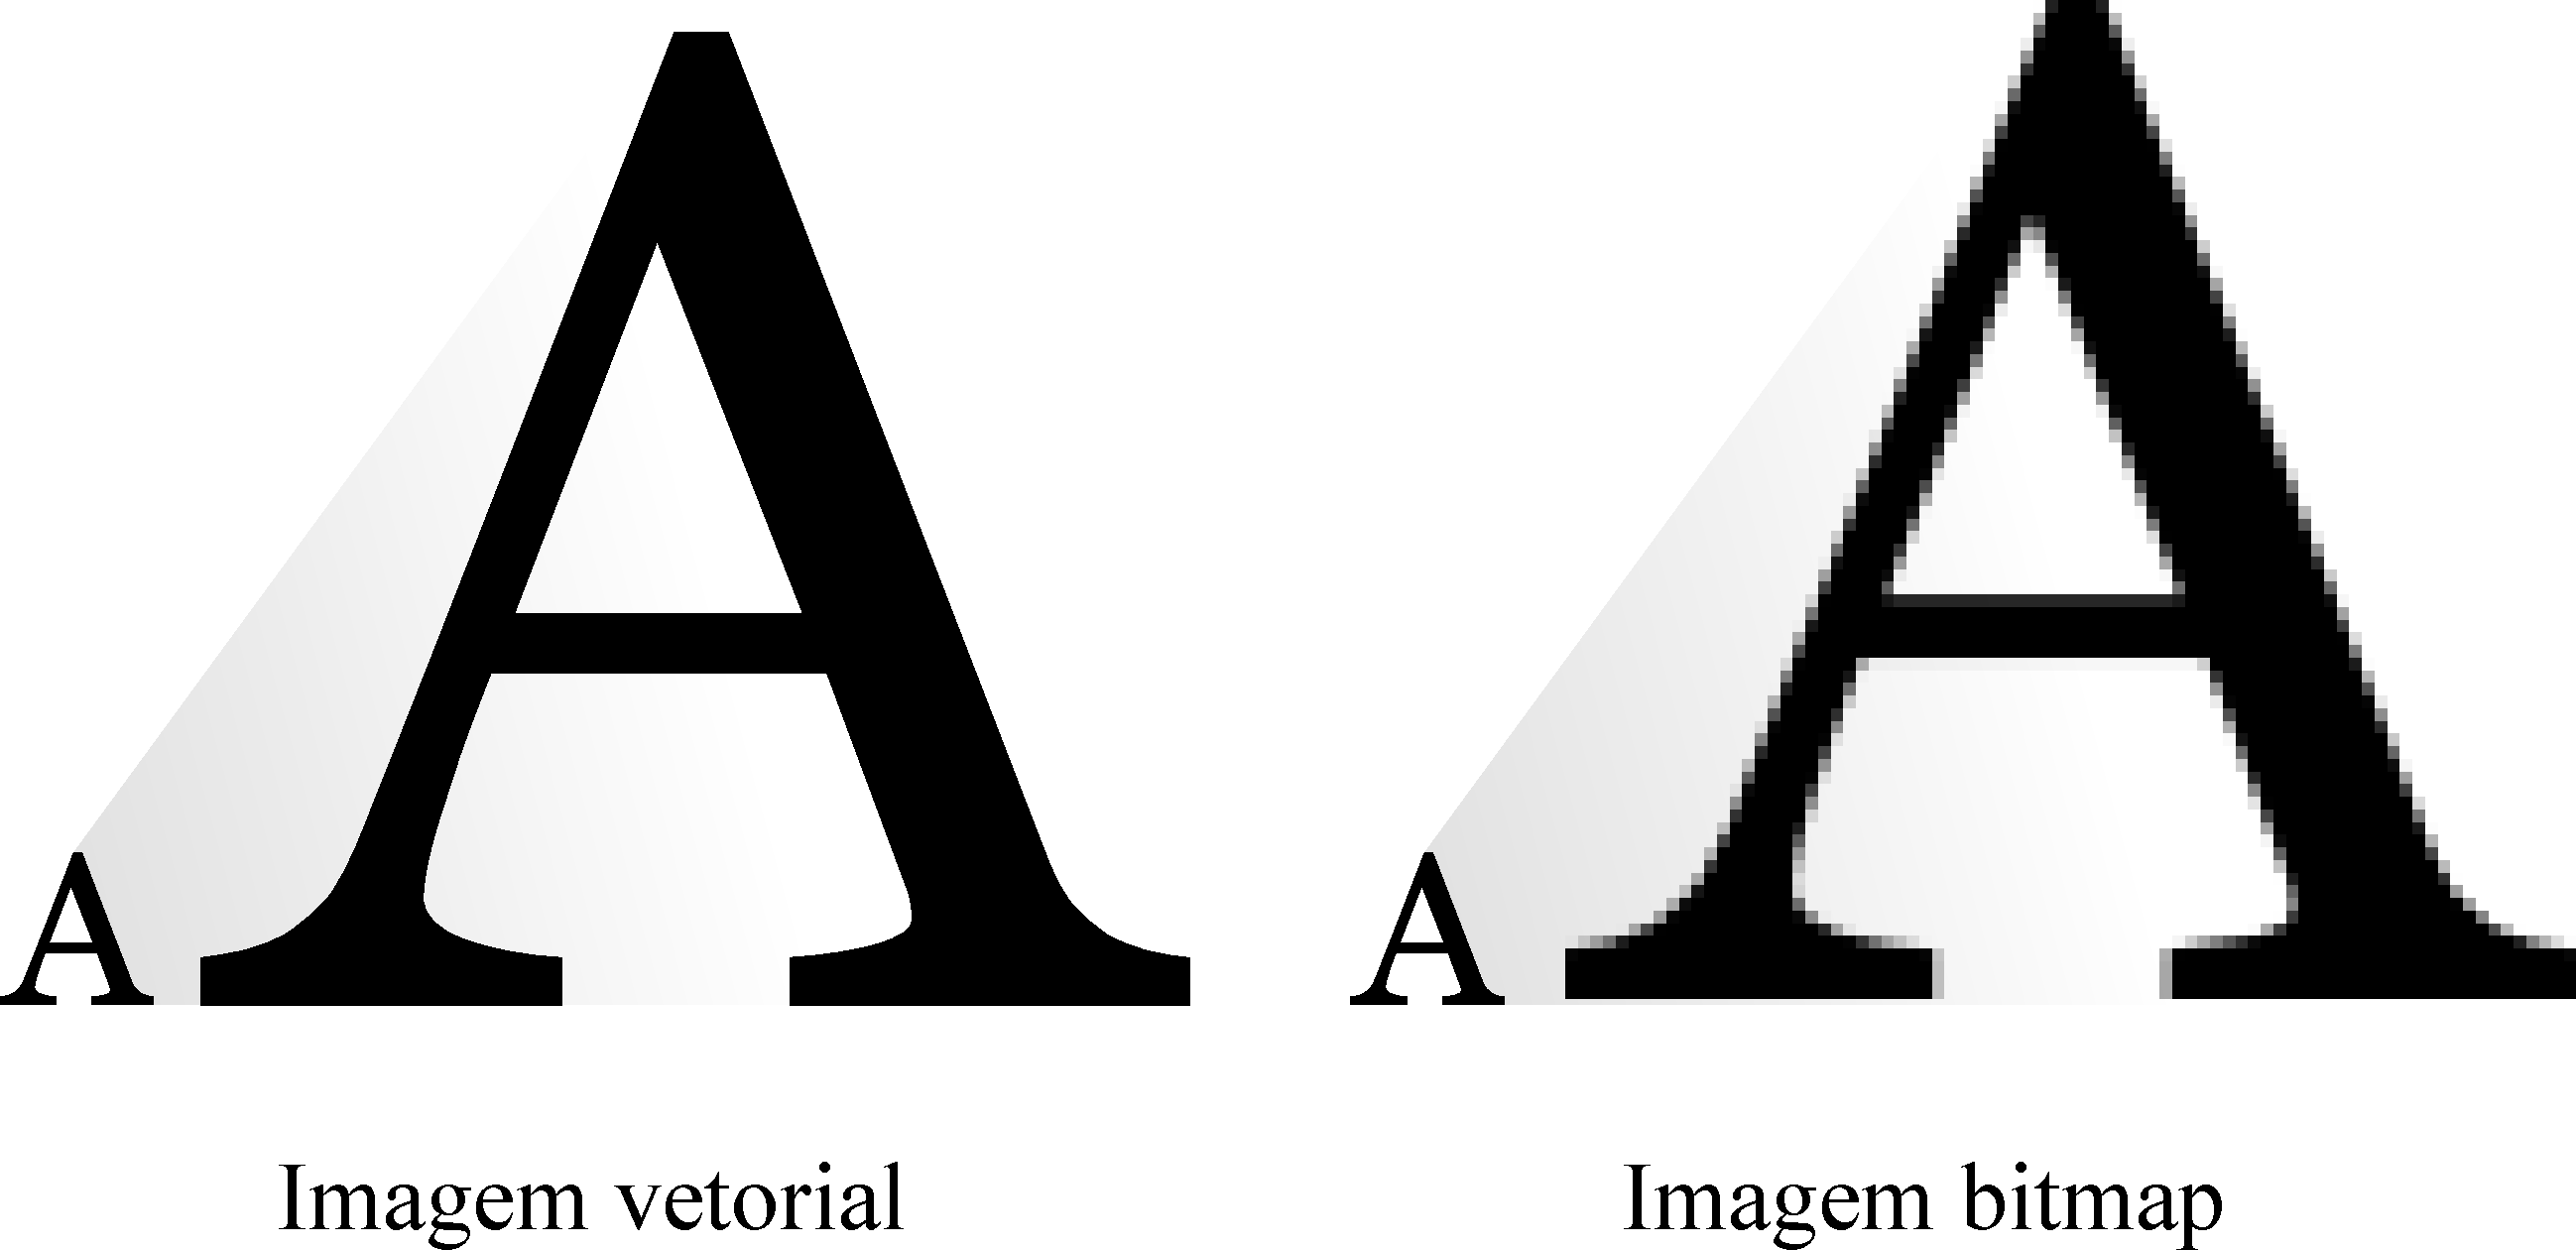
\includegraphics[height=4cm]{imagens/vetor_x_bitmap.pdf}
  \end{center}
  \caption{ Diferença entre uma imagem vetorial e uma imagem \textit{bitmap}.
    Uma imagem \textit{bitmap} perde a qualidade quando ampliada,
    o que não ocorre com uma imagem vetorial }
  \label{fig:vetor_x_bitmap}
\end{figure}

Quanto a cores, existem diversas padrões de representação, a
codificação RGB (sigla para \textit{Red},
\textit{Green}, \textit{Blue}) é a mais comum e define três bytes para armazenar,
respectivamente, o vermelho, o verde e o azul, cada uma sendo um inteiro na
faixa de 0 a 255. Outros padrões de representação são HLS
(sigla para \textit{Hue}, \textit{Lightness}, \textit{Saturation}),
HSB (sigla para \textit{Hue}, \textit{Saturation}, \textit{Brightness}),
HSV (sigla para \textit{Hue}, \textit{Saturation}, \textit{Value}), Hunter Lab,
CIE 1976 Lab e CMYK (sigla para \textit{Cian}, \textit{Magenta},
\textit{Yelow}, \textit{Black}), este último utilizado em mídias impressas.

Embora uma imagem \textit{bitmap} seja armazenada na RAM com todos os \textit{pixels} é comum,
por uma questão de economia de espaço e tempo de trasmissão, a compressão destes
arquivos. Entre todos os formatos de compressão os mais conhecidos são o GIF
(\textit{Graphics Inter-change Format}), o JPEG
(\textit{Joint Photographic Experts Group}) e
o PNG (\textit{Portable Network Graphics}).

Neste trabalho as imagens sempre serão \textit{bitmap}, com as cores codificadas
no padrão RGB e comprimidas no formato JPEG. As imagens serão tratadas como
equações, notacionadas na forma $ f(x,y) $, onde $ x $ e $ y $ são inteiros e indicam a
posição de um \textit{pixel} específico, e os pixels são interpretados como tuplas na
forma $ (r, g, b) $, onde $ r $, $ g $ e $ b $ pertencem ao subintervalo inteiro
de 0 a 255 e representam as cores vermelha, verde e azul respectivamente.

\section{Simplificação de imagens e extração de características}\label{sec:simplificacao_img}

Qualquer método de agrupamento depende sensivelmente do critério de semelhança
adotado nas comparações entre os elementos, será esse critério que, basicamente,
determinará a classe de cada elemento. O critério de semelhança deve ser baseado
em alguma característica mensurável e comparáveis entre sí, ou seja, deve haver
uma forma de se estabelecer a distância entre diferentes valores desta característica.
Esta distância determinará a semelhança entre os elementos, onde
quanto mais próximos mais semelhantes.

Em imagens existem diversas características que servem como critérios de
semelhança, do ponto de vista da percepção humana, estas características são
comumente ligados as cores, texturas ou formas presentes na imagen, ou ainda,
a uma combinação delas. Em relação as cores, medidas de histograma são as mais
populares; em texturas é comum a utilização de momentos do histograma de brilho,
matriz de co-ocorrência, granulometria e informações do aspectro de Fourier;
para formas se destacam os algorítimos de detecção de formas de interesse e os
momentos invariantes; uma abordagem mista de cores e formas é possível atravéz
de modelos de misturas gaussianas.

\section{Momentos invariantes como descritores de imagens}\label{sec:momentos_desc}

Supondo que uma forma particular estaja presente numa imagem $ A $, e que outra
bastante parecida esteja presente numa imagem $ B $, e que em relação a $ A $ a forma
em $ B $ está invertida, ou, para o exemplo ficar mais claro, que esta forma seja a
silhueta de um rosto, que em $ A $ está virado a esquerda e em $ B $ virado a direita,
como indicado na Figura \ref{fig:rostos}, é um objetivo particular deste trabalho que ambas
as imagens possuam descritores (características extraídas) bastante semelhantes,
senão identicos; afinal, em termos perceptivos, ou seja, em termos de significado
que um observador atribui as imagens, neste exemplo $ A $ e $ B $, ambas possuem a
figura de um rosto e estar cada um virado numa direção é uma caracterrística
marginal e não deve influenciar no agrupamento.

\begin{figure}[H]
  \begin{center}
    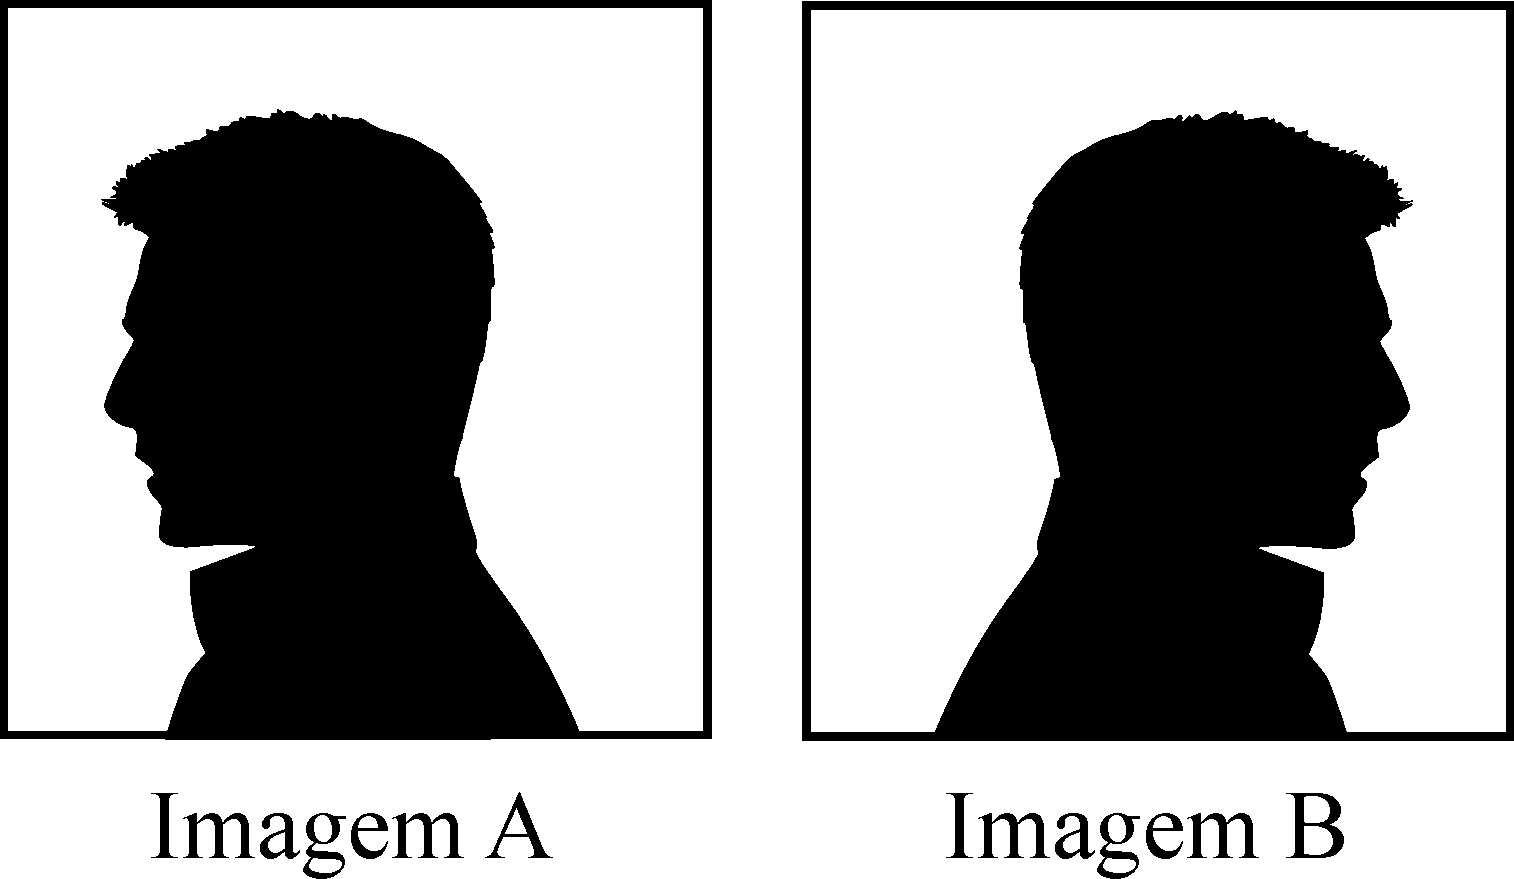
\includegraphics[height=4cm]{imagens/rostos.pdf}
  \end{center}
  \caption{ Duas imagens idênticas porém espelhadas.  }
  \label{fig:rostos}
\end{figure}

O mesmo pode ser dito para rotação, traslação e escala de formas em diferentes
imagens, o que se deseja é a forma em sí, algo como seu protótipo, independente
destas trasformações, como indica a Figura \ref{fig:carros_transformados}.
A pretenção é, ao se descartar estas transformações,
simular o que aparentemente é o comportamento natural de um indivíduo ao, sem
ajuda do computador, categorizar e agrupar imagens.

\begin{figure}[H]
  \begin{center}
    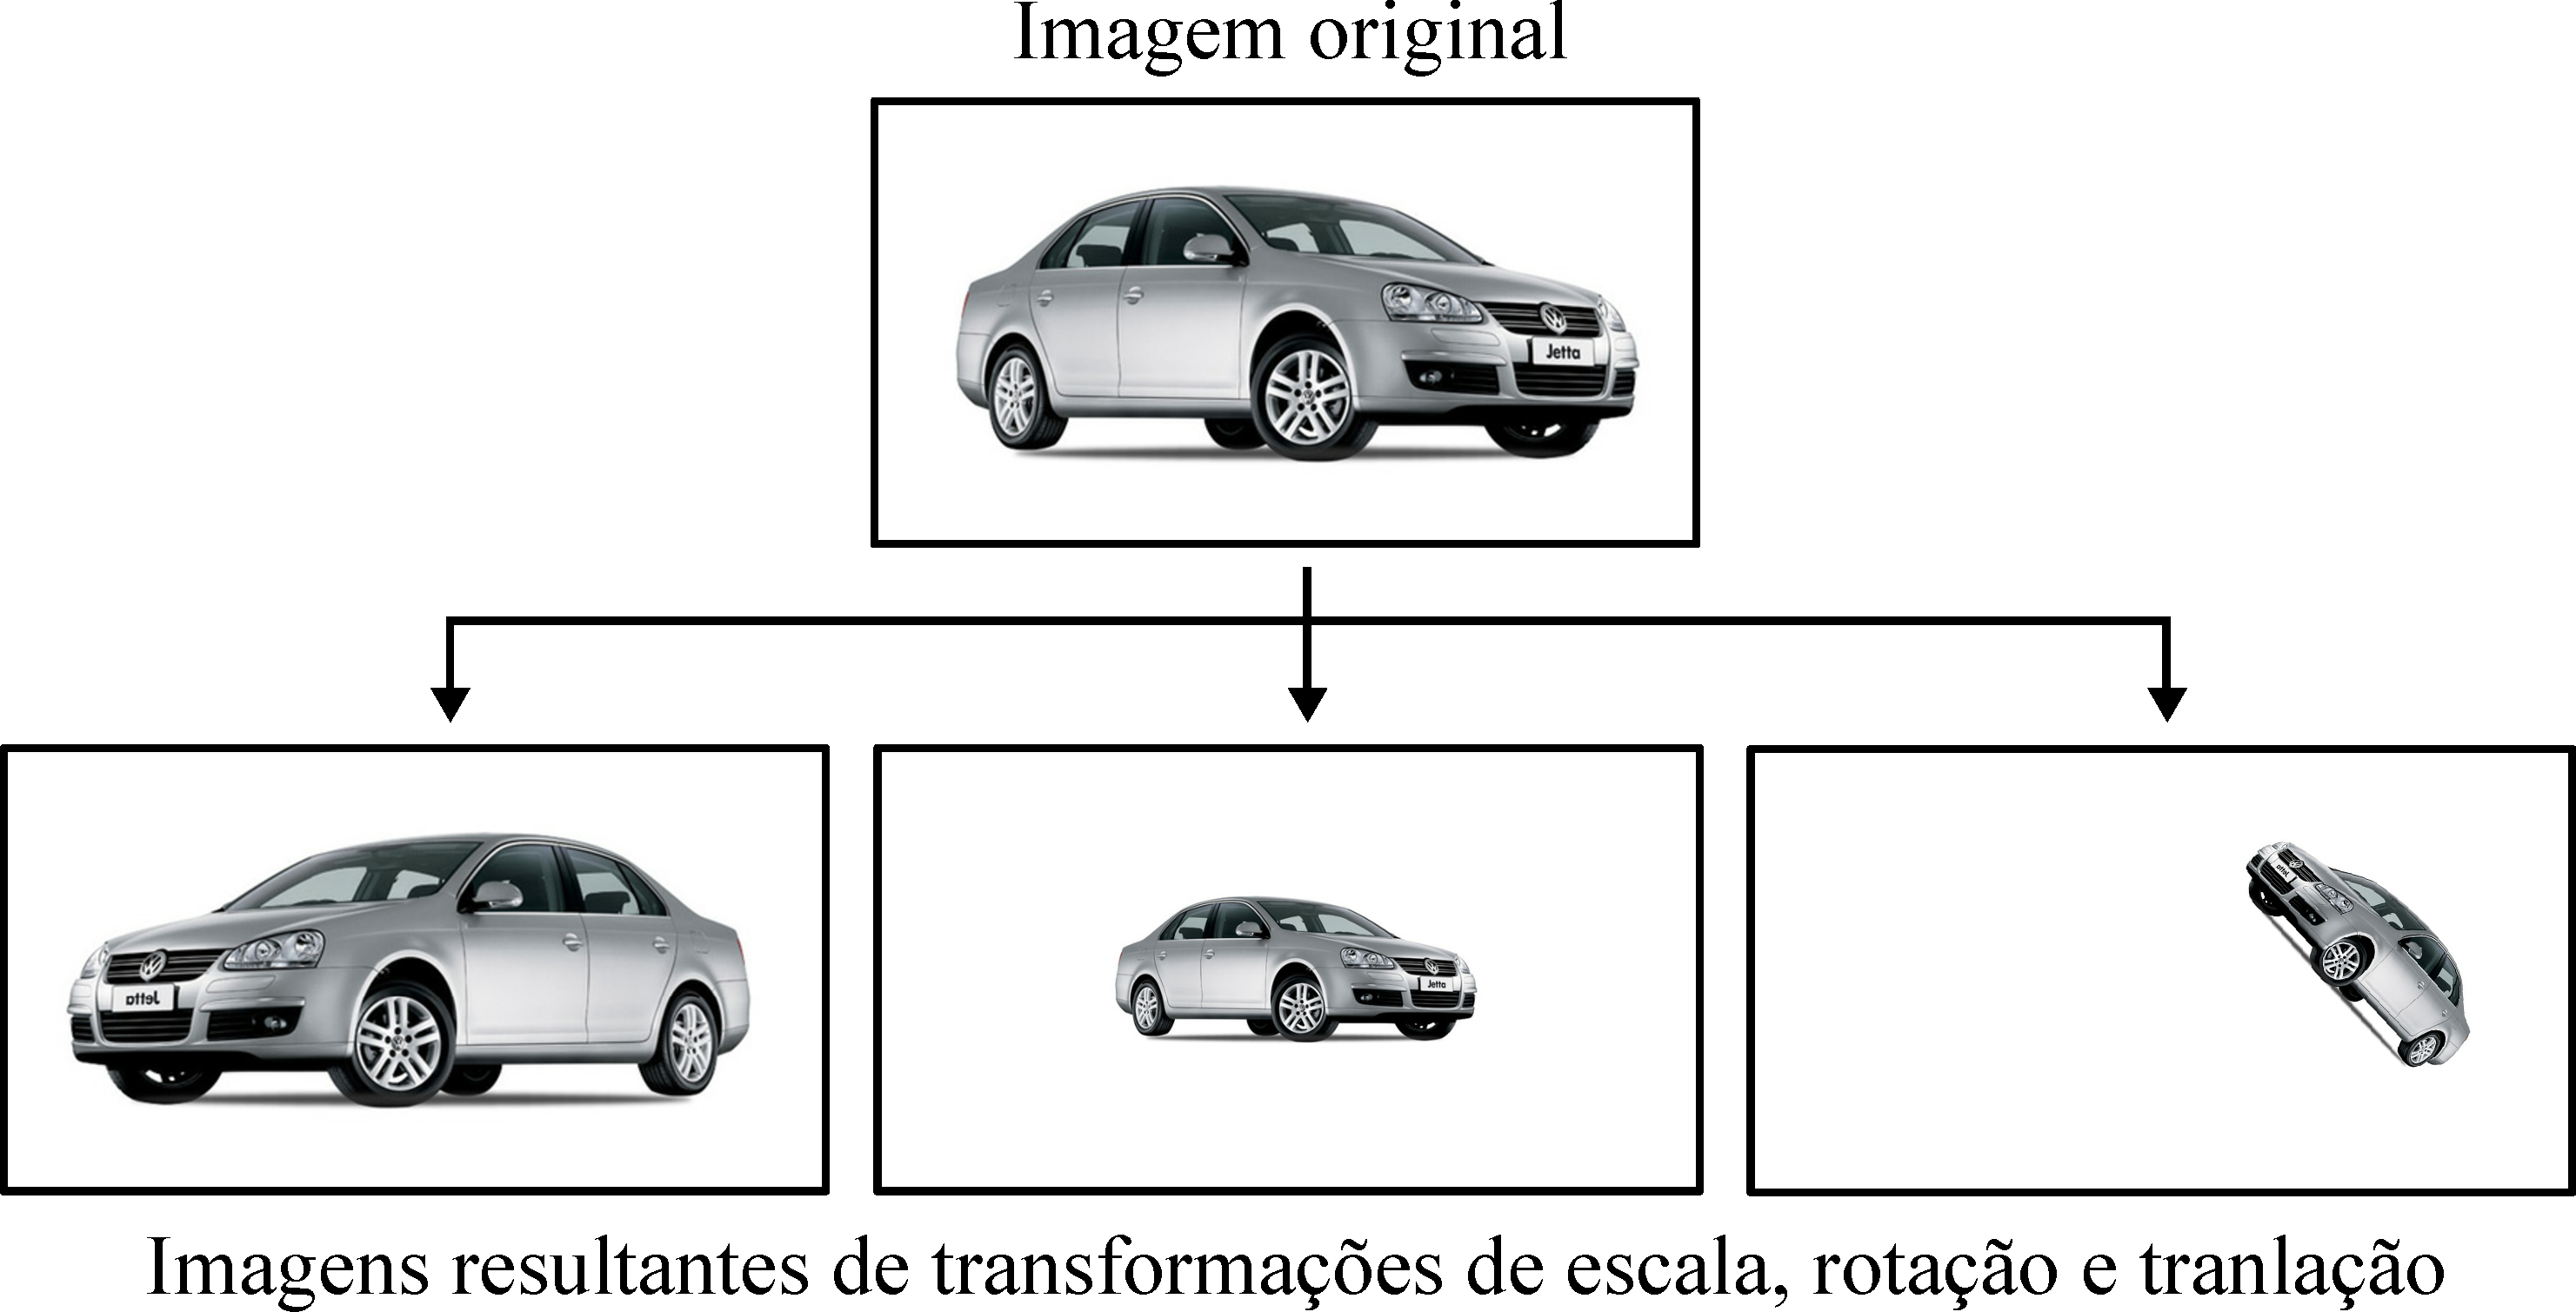
\includegraphics[height=7cm]{imagens/carros_transformados.pdf}
  \end{center}
  \caption{ Exemplos de transformações de rotação, translação e escala sobre
    uma imagem, e como elas não alteram a essência das formas presentes na
    imagem original. }
  \label{fig:carros_transformados}
\end{figure}

Um conjunto de descritores atende aos propósitos indicados acima, são os
descritores de Hu, mais comumente chamados de momentos invariantes. Os momentos
invariantes são um conjunto de sete descritores reais que independem de rotação,
translação ou escala, isto é, quando aplicados a uma forma qualquer retornará
os mesmos valores se aplicado a outra forma resultande de uma das três
transformações citadas, ou até mesmo de uma combinação delas.

\subsection{Formulação matemáticas dos momentos invariantes}\label{sec:momentos_mat}

Passemos então agora para formalização matemática desses momentos.

O momento bidimensional de ordem $ (p+q) $ é dado pela
equação \ref{eq:mm_bid_cont}:

\begin{equation}\label{eq:mm_bid_cont}
m_{pq} = \iint x^p y^q f(x, y) \mathrm{d}x \mathrm{d}y, p, q \in
\end{equation}

A equação num domínio discreto, pode ser reescrita na forma:

\begin{equation}\label{eq:mm_bid_disc}
m_{pq} = \sum_{x, y} x^p y^q f(x, y), p, q \in
\end{equation}

A massa total da função $ f(x, y) $ é determinado pelo
momento $ m_{00} $, conforme a equação \ref{eq:mm_bid_m00}:

\begin{equation}\label{eq:mm_bid_m00}
m_{pq} = \sum_{x, y} f(x, y), p, q \in
\end{equation}

Existe um ponto no qual a aplicação pontual da massa total gera o mesmo momento
que a massa distribuída, este ponto é dito centroide de $ f(x, y) $ e suas
coordenadas $ x $ e $ y $ são dadas pela equação \ref{eq:ct_xy}:

\begin{subequations}\label{eq:ct_xy}
\begin{align}
    \bar{x} = \frac{1}{ m_{00} } \sum x f(x, y) = \frac{ m_{10} }{ m_{00} } \\
    \bar{y} = \frac{1}{ m_{00} } \sum y f(x, y) = \frac{ m_{01} }{ m_{00} }
\end{align}
\end{subequations}

O momento central é obtido se deslocando a imagem para o centroide,
da seguinte forma:

\begin{equation}\label{eq:mm_ctr}
\mu_{pq} = \sum_{x, y} (x - \bar{x})^p (y - \bar{y})^q f(x, y)
\end{equation}

Ainda é necessário normalizar o momento para que os valores resultantes não sejam
extremos a ponto de serem ignorados pelo sistema de reconhecimento de padrões. O
momento central de ordem $ (p+q) $ normalizado é obtido dividindo o momento
central de $ y $ mesma ordem por um fator definido por $ \mu_{00}^\gamma $ ,
conforme indicado pela equação \ref{eq:mm_norm}:

\begin{subequations}\label{eq:mm_norm}
\begin{align}
    \gamma = 1 + \frac{ p + q }{2} \\
    \eta_{pq} = \frac{ \mu_{pq} }{ \mu_{00}^\gamma }
\end{align}
\end{subequations}

A partir dessas equações são estabelecidos sete momentos invariantes à translação,
 rotação e escala, chamados de momentos de Hu, ou descritores de Hu. São eles:

\begin{subequations}\label{eq:mmt}
\begin{align}
  \varphi_1 = \eta_{20} + \eta_{02} \\
  \varphi_2 = (\eta_{20} - \eta_{02})^2 + 4\eta_{11}^2\\
  \varphi_3 = (\eta_{30} - 3\eta_{12})^2 + (3\eta_{21} - \eta_{03})^2\\
  \varphi_4 = (\eta_{30} + \eta_{12})^2 + (3\eta_{21} + \eta_{03})^2 \\
%
  \begin{tabular}{r c l}
    \(\varphi_5\) & \(=\) & \((\eta_{30} - 3\eta_{12})(\eta_{30} + \eta_{12}) \left[ (\eta_{30} + \eta_{12})^2 - 3(\eta_{21} + \eta_{03})^2 \right]\) \\
                  & \(+\) & \((3\eta_{21} - \eta_{03})(\eta_{21} + \eta_{03}) \left[ 3(\eta_{30} + \eta_{12})^2 - (\eta_{21} + \eta_{03})^2 \right]\)
  \end{tabular}\\
%
  \begin{tabular}{r c l}
    \(\varphi_6\) & \(=\) & \((\eta_{20} - \eta_{02})\left[ (\eta_{30} + \eta_{12})^2 - (\eta_{21} + \eta_{03})^2 \right]\)\\
                  & \(+\) & \(4\eta_{11}(\eta_{30} - \eta_{12})(\eta_{21} + \eta_{03})\)
  \end{tabular}\\
%
  \begin{tabular}{r c l}
    \(\varphi_7\) & \(=\) & \((3\eta_{21} - \eta_{30})(\eta_{30} + \eta_{12})\left[ (\eta_{30} + \eta_{12})^2 - 3(\eta_{21} + \eta_{03})^2 \right]\)\\
                  & \(+\) & \((3\eta_{12} - \eta_{03})(\eta_{21} + \eta_{03})\left[ 3(\eta_{30} + \eta_{12})^2 - (\eta_{21} + \eta_{03})^2 \right]\)
  \end{tabular}
\end{align}
\end{subequations}

Observe que os momentos são definidos para um ponto de valor discreto, isto implica que
devemos abandonar qualquer descriçao vetorial de cores, neste caso, devemos
passar uma cor do formato RGB para seu tom de cinza. Neste trabalho o tom de
cinza para uma cor RGB é o valor médio para os canais vermelhor, verde e azul.

\section{Binarização de imagens}\label{sec:binarizacao_img}

Mesmo que os momentos invariantes sejam, a princípio, bons descritores, eles
não podem ser extraídos sem que a imagem tenha passado por algumas
transformações. Estas transformações não são obrigatórias, isto é, não são
restrições necessárias a aplicação dos momentos, mas são transformações que
fazem sentido no processo de agrupamento, mais especificamente, no subprocesso
de extração de características relevantes.

É perfeitamente válido supor que nem todas os \textit{pixels} de uma imagem sejam
relevantes, ou no mínimo, que determinados \textit{pixels} são mais relevantes
que outros, estes \textit{pixels} mais relevantes podem ser interpretados
como regiões de interesse, isto é, regiões que despertam maior atenção dos
observadores. Em suma, podemos dividir a imagem em duas regiões, uma de
interesse chamada de primeiro plano (\textit{foreground}) e outra que pode ser
negligenciada chamada plano de fundo (\textit{background}), como no exemplo
da Figura \ref{fig:girafa_limiarizacao}. A separação entre
essas duas regiões é chamado de limiarização, ou ainda, remoção de fundo.

\begin{figure}[H]
  \begin{center}
    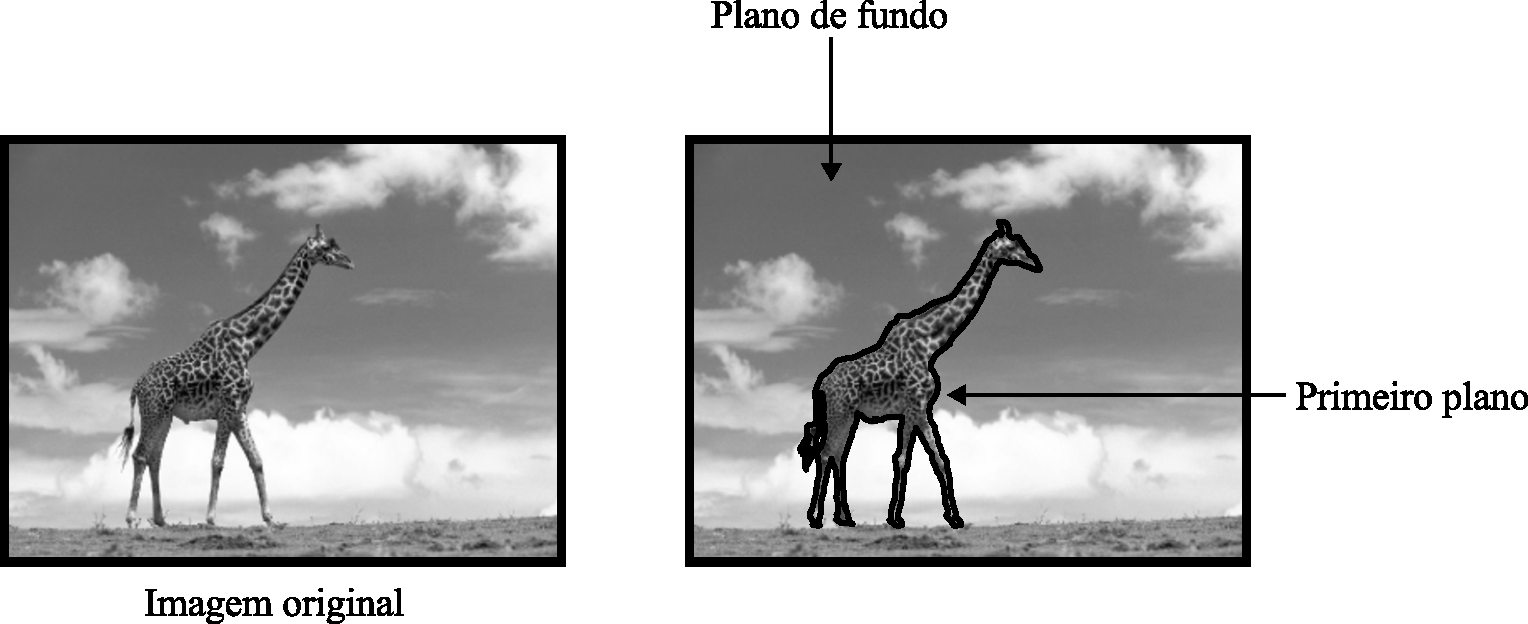
\includegraphics[height=6cm]{imagens/girafa_limiarizacao.pdf}
  \end{center}
  \caption{ Imagem com o primeiro plano e o plano de fundo destacados. }
  \label{fig:girafa_limiarizacao}
\end{figure}

Extrair da imagem os momentos invariantes apenas do primeiro plano
torna os descritores mais interessantes para classificação, afinal, os valores
ficam restritos apenas a região de maior interesse, sendo o plano de fundo
totalmente ignorado na extração destas características.

Outro ponto a ser considerado, como visto na seção anterior, é que
a extração dos momentos depende da intensidade de
cada \textit{pixel}, de modo que uma variação na intensidade de um \textit{pixel}
interfere no resultado dos momentos. Como agora apenas o primeiro plano é
aplicado na extração, apenas as variações de intensidade nesta região são
consideradas; contudo, estas variações podem em determinadas ocasiões gerar
momentos muito distintos para regiões que, morfologicamente, são bem parecidas.
Suponha o caso de, por exemplo, duas imagens que no primeiro plano apresentam a
figura de uma flor, como na Figura \ref{fig:flor_mmt}, na primeira a flor
tem a coloração clara, e na segunda escura, ao aplicar o momento sobre estas
duas imagens, mesmo que tenham uma forma bem parecida, teremos resultados
significativamente diferentes para os momentos das duas. É desejável eliminar
este tipo de discrepância, isto é possível tornando todas as informações da
primeiro plano homogêneas, ou seja, fazer com que cada \textit{pixel} do
primeiro plano tenha o mesmo peso para extração dos momentos. Esta homogenização
sobre uma imagem já limiarizada é chamada de
binarização, isto porque teremos duas regiões, uma irrelevante onde
cada \textit{pixel} terá o valor nulo, e outra relevante onde cada \textit{pixel}
terá seu máximo valor.

\begin{figure}[H]
  \centering

  \begin{subfigure}{0.3\textwidth}
    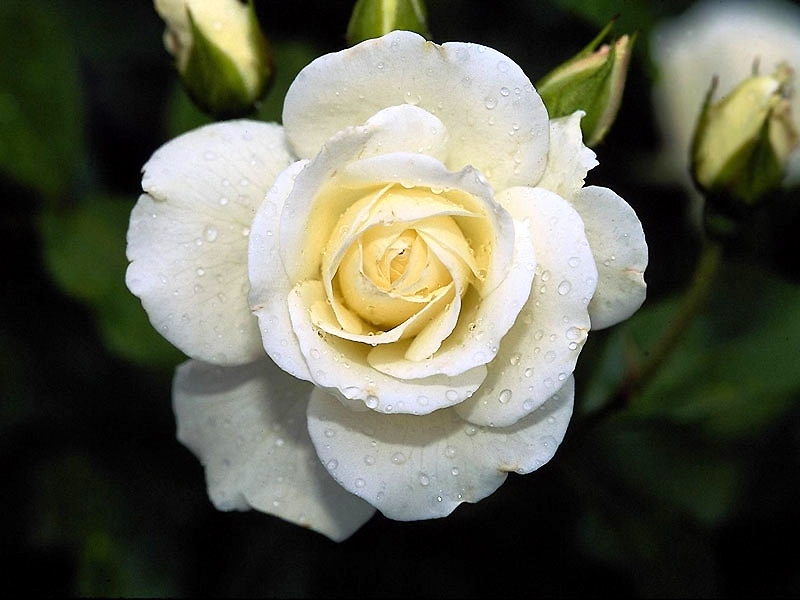
\includegraphics[width=\textwidth]{imagens/flor_branca.jpg}
    \caption{Rosa branca}
    \label{fig:flor1}
  \end{subfigure}~
  \begin{subfigure}{0.3\textwidth}
    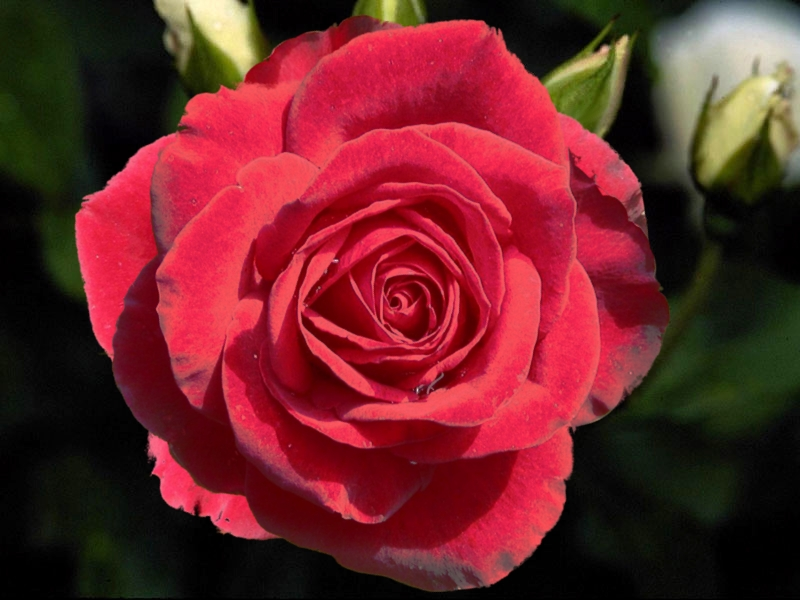
\includegraphics[width=\textwidth]{imagens/flor_vermelha.jpg}
    \caption{Rosa vermelha}
    \label{fig:flor2}
  \end{subfigure}~

  \begin{subfigure}{0.3\textwidth}
    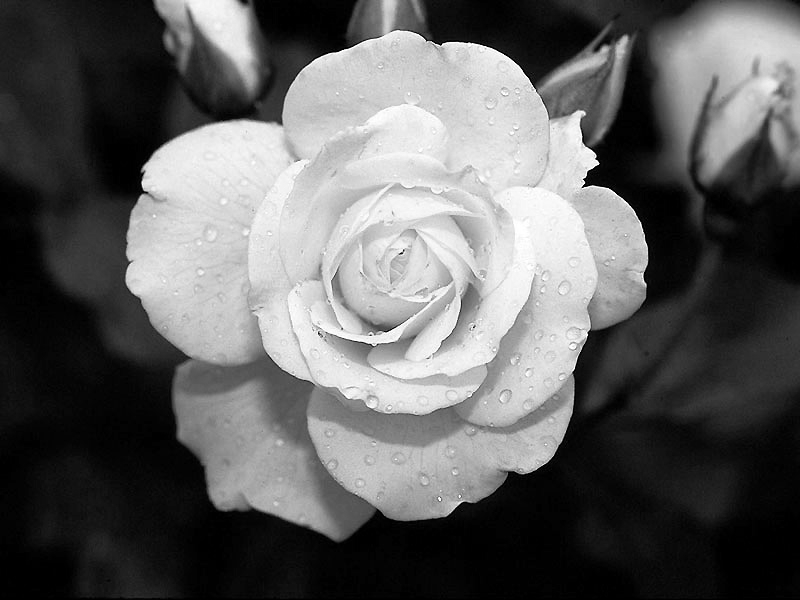
\includegraphics[width=\textwidth]{imagens/flor_branca_pb.jpg}
    \caption{Rosa branca em tons de cinza}
    \label{fig:flor3}
  \end{subfigure}~
  \begin{subfigure}{0.3\textwidth}
    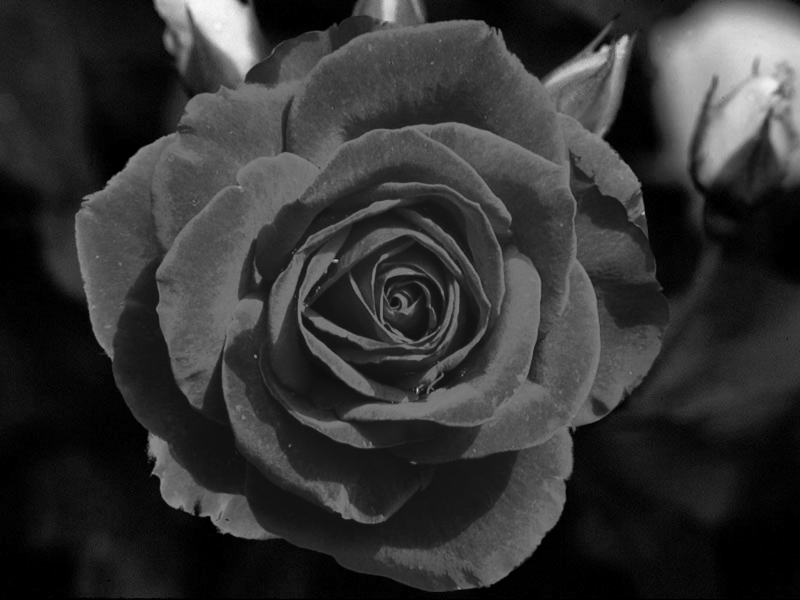
\includegraphics[width=\textwidth]{imagens/flor_vermelha_pb.jpg}
    \caption{Rosa vermelha em tons de cinza}
    \label{fig:flor4}
  \end{subfigure}

  \caption{ Imagens visualmente semelhantes mas com relativa diferença nos
    valores dos momentos devido as grande diferença de tons no primeiro plano. }
  \label{fig:flor_mmt}
\end{figure}

Binarizar uma imagem, o que implicitamente também implica em limiarizá-la, é
um processo bem simples e pode ser feito apenas como base no histograma. O que
se deseja é anular todos os \textit{pixels} abaixo de um limiar e
potencializar os que estão acima dele. Como indicado no Algoritmo \ref{alg:binarizacao_imagem}:

\begin{algorithm}[H]
\caption{Binarização de uma imagem}\label{alg:binarizacao_imagem}
\SetAlgoRefName{alg:binarizacao_imagem}
\Entrada{$ f(x, y) $ , $ l $ }
\Inicio{
  \ParaCada{$ p \in f(x, y) $}{
    \eSe{$ p < l $}{
      $ p \gets 0 $
    }{
      $ p \gets 255 $
    }
  }
}
\end{algorithm}

Contudo, o Algorítimo \ref{alg:binarizacao_imagem} não indica como definir o limiar
ótimo, isto é, aquele que melhor separa o primeiro plano do plano de fundo, esta
operação é realizada, neste trabalho, através do método de Otsu, descrito na próxima seção.

\section{Método de Otsu}\label{sec:metodo_otsu}

O método de Otsu é um método de \textit{thresholding} global, isto é, o valor obtido é
uma constante, para escolha do melhor limiar. A base deste método é sua interpretação
do histograma como como uma função de densidade de probabilidade
discreta, da seguinte maneira:

\begin{equation}\label{eq:histograma_norm}
  p_r(r_q) = \frac{n_q}{n}, q = 0, 1, 2, ..., L-1
\end{equation}

Onde:

\begin{itemize}
  \item $ n $ é o total de \textit{pixels} da imagem;
  \item $ n_q $ é o total de \textit{piixels} que tem intensidade $ r_q $ e
  \item $ L $ é o total de níveis de intensidade na imagem.
\end{itemize}

O método de Otsu escolhe o limiar de valor $ k $, tal que $ k $ é um nível de
intensidade que divide o histograma em duas classes
$ C_0 = [0, 1, ..., k-1] $ e $ C_1 = [k, k+1, ..., L-1] $, e que maximise a
variância $ \sigma_{B}^2 $ definida como:

\begin{equation}\label{eq:maximizacao_variancia}
  \sigma_{B}^2 = \omega_0(\mu_0 - \mu_T)^2 + \omega_1(\mu_1 - \mu_T)^2
\end{equation}

Sendo:

\begin{subequations}\label{eq:somatorios_maximizacao}
\begin{align}
  \omega_0 = \sum_{q=0}^{k-1} p_q(r_q)\\
  \omega_1 = \sum_{q=k}^{L-1} p_q(r_q)\\
     \mu_0 = \sum_{q=0}^{k-1} \frac{qp_q(r_q)}{\omega_0}\\
     \mu_1 = \sum_{q=k}^{L-1} \frac{qp_q(r_q)}{\omega_1}\\
     \mu_T = \sum_{q=0}^{L-1} qp_q(r_q)
\end{align}
\end{subequations}

O resultado da binarização com limiar ajustado segundo o método de Otsu pode
ser observado na Figura \ref{fig:bin_otsu}

\begin{figure}[H]
  \centering

  \begin{subfigure}{0.3\textwidth}
    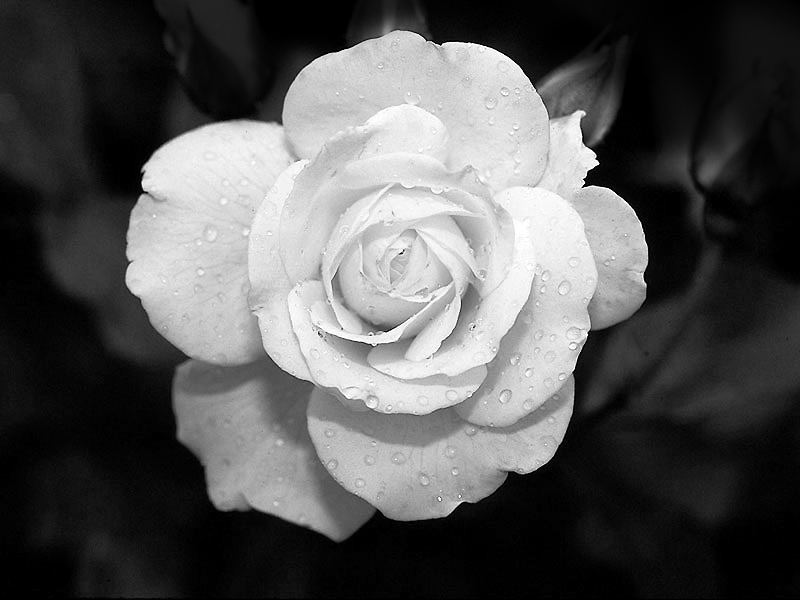
\includegraphics[width=\textwidth]{imagens/flor_branca_pb2.jpg}
    \caption{Imagem original}
    \label{fig:flor1}
  \end{subfigure}~
  \begin{subfigure}{0.3\textwidth}
    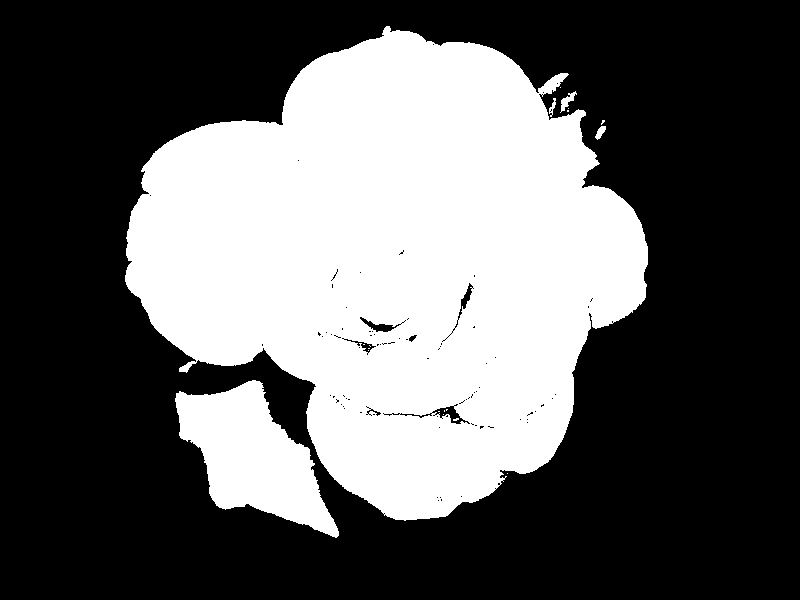
\includegraphics[width=\textwidth]{imagens/flor_branca_pb2_lm.jpg}
    \caption{Imagem binarizada}
    \label{fig:flor2}
  \end{subfigure}~

  \caption{ Imagem binarizada com limiar definito pelo método de Otsu. }
  \label{fig:bin_otsu}
\end{figure}

\section{Resumo do processo de extração de características}
\label{sec:resumo_extracao_caracteristicas}

Como discutido nas seções anteriores deste capítulo, os momentos invariantes
foram eleitos como os descritores a serem utilizadas para determinar a
similaridade entre as imagens, contudo, estes descritores são extraídos somente
após as imagens terem passado por determinadas transformações que visam
simplificá-las e potencializar as regiões de maior interesse, e assim, produzir
valores mais significativos para os momentos. As transformações  aplicadas as
imagens são a dessaturação e a binarização, nesta ordem.

Podemos resumir visualmente o processo de extração de característica na
Figura \ref{fig:extracao_caracteristicas}:

\begin{figure}[H]
  \begin{center}
    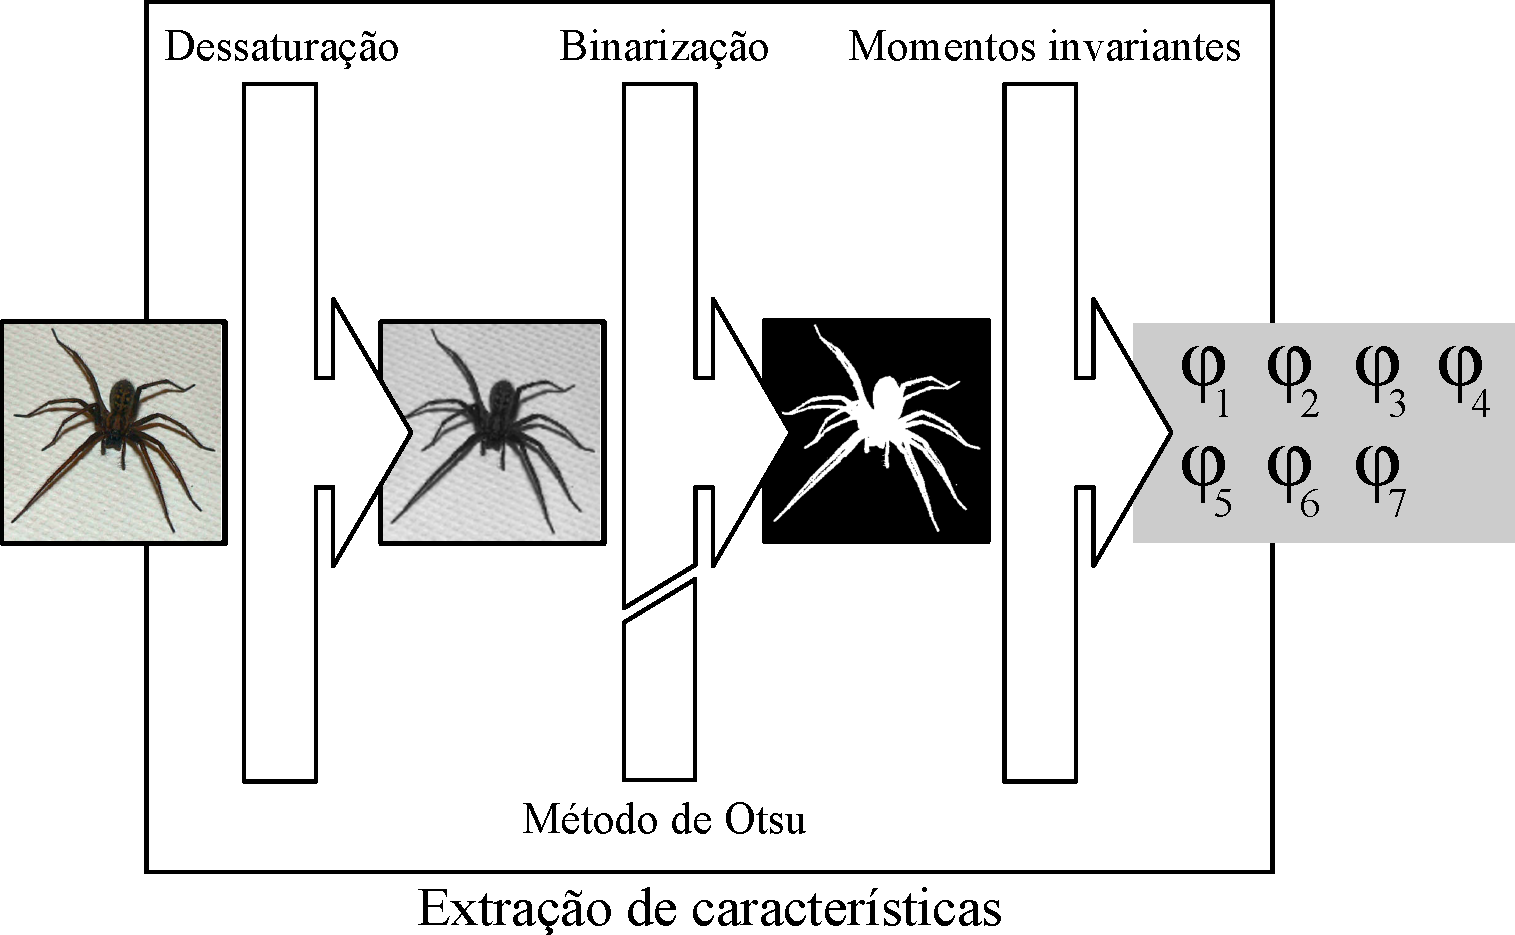
\includegraphics[height=8cm]{imagens/extracao_caracteristicas.pdf}
  \end{center}
  \caption{ Esquema do processo de extração de caracteristicas. }
  \label{fig:extracao_caracteristicas}
\end{figure}
